\documentclass{ximera}%handout option removes answers

\usepackage{animate}
\usepackage{tikz}
\usepackage{pgfplots}
\usepackage{pst-3dplot}
\usepackage{pst-solides3d}
\usepackage{pst-math}
\usetikzlibrary{fpu,shadows.blur,shapes.symbols,patterns}
\usetikzlibrary{topaths,intersections,calc,shapes.geometric,arrows,through, positioning}
\usepackage{fp}

\title{Linear ODEs}
\author{Timothy All}

\begin{abstract}
  ODEs and stuff
\end{abstract}

\begin{document}
\maketitle



\begin{problem} Which of the following ODEs is linear?
\begin{multipleChoice}
\choice{$y'' - y^2 = 0$}
\choice{$\sin y = y'$}
\choice[correct]{$y''+t y = 0$}
\choice{$\sqrt{1+y^2}=y'$}
\end{multipleChoice}
\end{problem}

\begin{problem}
   If $y'' - y = 0$, then $y = \answer{c_1 \cosh(t) + c_2 \sinh(t)}$ where $c_1$ and $c_2$ are constants.
\end{problem}

\begin{example} Model the motion of a coupled spring-mass system.

\begin{image}
%\begin{animateinline}[controls]{18}
%\multiframe{11}{rTick=0+.1}{
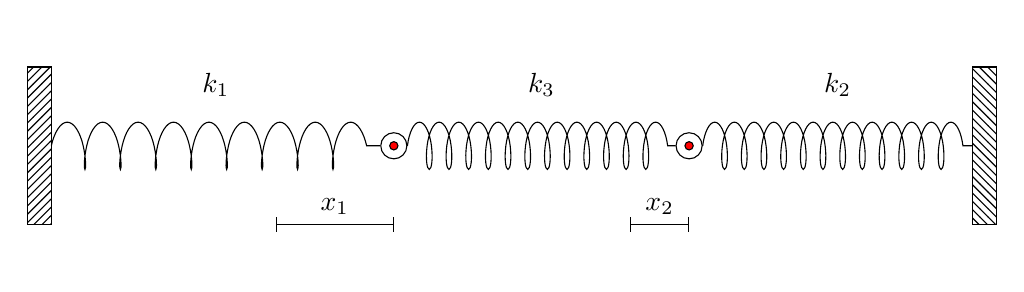
\begin{tikzpicture}[x=1.5cm]
\useasboundingbox (-.1,-1.5) rectangle (8.1,1.5);
\pgfmathsetmacro\rTick{1}
\pgfmathsetmacro\a{2+\rTick}
\pgfmathsetmacro\b{5+\rTick/2}
\pgfmathsetmacro\oa{\a*3/2}
\pgfmathsetmacro\ab{(\b-\a)}
\pgfmathsetmacro\bo{8-\b}

\node[circle,draw] (A) at (\a,0) {};%2
\node[circle,draw] (B) at (\b,0) {};%5
\draw [fill=red] (A) circle (1.5pt);%
\draw [fill=red] (B) circle (1.5pt);%

\draw [decoration={aspect=0.3, segment length=\oa mm, amplitude=3mm,coil},decorate] (.1,0)--(A) node[midway,above=.5] {$k_1$};%
\draw [decoration={aspect=0.3, segment length=\ab mm, amplitude=3mm,coil},decorate] (A)--(B) node[midway,above=.5] {$k_3$};%
\draw [decoration={aspect=0.3, segment length=\bo mm, amplitude=3mm,coil},decorate] (B)--(7.9,0) node[midway,above=.5] {$k_2$};%

\draw [pattern=north east lines] (-.1,-1) rectangle (.1,1);%

\draw [pattern=north west lines] (7.9,-1) rectangle (8.1,1);

\draw [|-|] (2,0)++(-90:1) --+ (0:\rTick) node[midway,above] {$\answer{x_1}$};
\draw [|-|] (5,0)++(-90:1) --+ (0:\rTick/2) node[midway,above] {$x_2$};

\end{tikzpicture}
%}
%\end{animateinline}

\end{image}

\begin{explanation}
Newton's second law says that $F= \answer{m \cdot a}$


\end{explanation}


\end{example}

Plz work

\[ \graph{ax^2,a=.5} \]


\end{document}
